\section{LaTeX online}

\begin{frame}[allowframebreaks]
\frametitle{\LaTeX{} online}

\centering
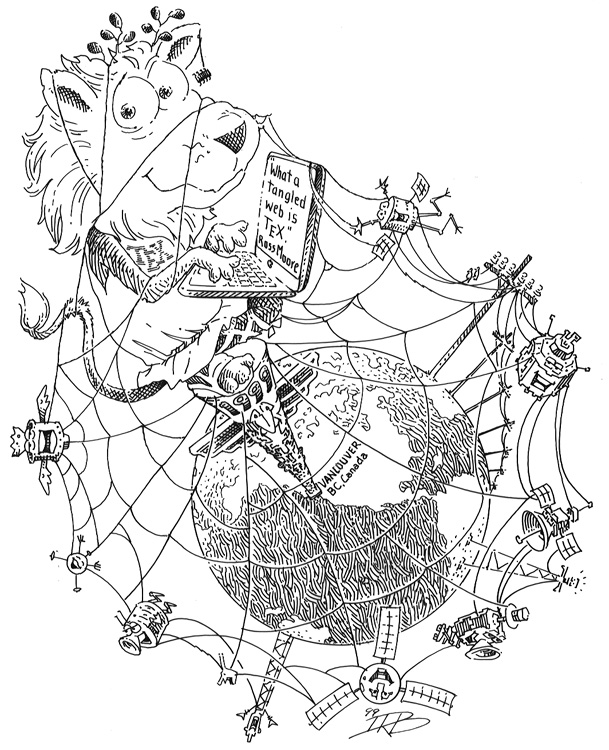
\includegraphics[width=0.4\linewidth,height=0.7\textheight,keepaspectratio]{figures/lion05.png}

\framebreak

\begin{description}
\item[\hrefcolor{https://www.overleaf.com/}{Overleaf}] editor \LaTeX{} colaborativo (em 2017 o Overleaf adquiriu o ShareLaTeX)
\item[\hrefcolor{https://cocalc.com/doc/latex-editor.html}{Cocalc}] é uma plataforma de computação na nuvem com suporte a \LaTeX{}, 
Markdown, HTML, R, Octave, Cython, Julia, Python, ambiente Linux, Jupyter Notebook.
\item[\hrefcolor{https://latexbase.com/}{\LaTeX{} Base}] editor online
\item[\hrefcolor{https://papeeria.com/}{Papeeria}] editor online
\item[\hrefcolor{https://listoffreeware.com/list-of-best-free-online-latex-editors/}{outros}]
\end{description}


Controle de versão
\begin{itemize}
\item Git, Mercurial, Subversion, CVS, etc
\item servidor remoto ou local
\end{itemize}
\end{frame}
